\subsection{Existence of Quark Gluon Plasma}
\subsection{Relativistic Heavy Ion Collision Geometry}
\textcolor{red}{include a figure of the lightcone diagram for heavy ion collisions}
\textcolor{red}{include explanation of pseudorapidity in heavy ion collisions}
\subsubsection{Initial State and Bjorken Energy Density}
The experimental measurement of the mean transverse energy as a function of rapidity of the final collision particles has direct link to the initial state of these heavy ion collisions. 
In an idealized picture of heavy ion collisions, the energy density of the initial collision just prior to hydrodynamic flow could be found directly from measuring the average energy as a function of rapidity of the final state particles in the central rapidity plateau region, assuming the QGP behaves as an ideal boost invariant relativistic fluid and there are little final state effects \cite{bjorken_energy_density}. 
Here Bjorken estimated the initial energy density that forms in the central rapidity region between two receeding Lorentz contracted nuclei using the mean number of charged particles as a function of rapidity for nucleon-nucleon collisions measured in data, the average energy per nucleon from collision data, and assumed that for a collision system of nuclei, the average energy as a function of rapidity should be additive. 
In his initial estimates, the energy density in the central rapidity region for A+A collisions should be on the order of 1 to 10 GeV/fm$^3$ \cite{bjorken_energy_density}.
This relationship has since been used to provide experimental measurements of \detdeta, \: and subsequent measurements of $dE_{T}/dy$, and infer mean initial energy densities for these collision systems using the following relationship: 
\begin{equation}
    \epsilon_{Bj} = \frac{dE_{T}}{dy} \frac{1}{\tau_{0} \pi R^2}
\end{equation}
where $\tau_{0}$ is the formation time and $\pi R^2$ is the effective area of the collision. 

From previous measurements of the energy density via the mean transverse energy of final state particles of the heavy ion collisions, the energy density in central collisions of \auau \: ions at \sqsntwo \: using this Bjorken energy density relationship  has been measured to be greater than 4 GeV/fm$^3$ \cite{STAR_detdeta,PHENIX_200gev}. 
In comparison, the energy density inside of a typical hadron is about 500 MeV/fm$^3$ \cite{Busza_2018}. 
Therefore, from first measurements of this Bjorken energy density in heavy ion collisions, the energy density was found to be much greater than the energy density of typical confined nuclear matter.

Measurements of the mean transverse energy and resulting initial collision energy density have been studied by many detectors at RHIC and the LHC for both heavy ion collisions and small systems such as $p+p$, $p+Pb$ and $d+Au$ \cite{PHENIX_detdeta,STAR_detdeta,cms_pbpb_detdeta,alice_detdeta,cms_pPb_detdeta,atlas_detdeta}. 
These experiments have for the large part employed two distinct methods of measuring total transverse energy, the first method has been used by ATLAS and CMS \cite{cms_pbpb_detdeta,atlas_detdeta}, where the transverse energy in the detectors' calorimeters are measured and these measurements are corrected for detector effects, limits in detector acceptance and detector hadronic response back to the truth \detdeta of the collisions, which includes both hadronic and electromagnetic energy contributions. 
This method works best in calorimeter systems with a large number of radiation/interaction lengths therefore allowing for the majority if not all of the collision energy to be captured by the detector. 
This methodology was also employed by PHENIX \cite{PHENIX_detdeta} without a hadronic calorimeter; instead PHENIX was able to correct back to the truth \detdeta from a combination of electromagnetic energy, minimum ionizing particles and a small contribution from hadronic showers. 
The second method has been used by STAR and ALICE \cite{STAR_detdeta,alice_detdeta}, in which the hadronic component of the transverse energy is measured using the tracking subsystems and the electromagnetic component of the transverse energy is measured using the calorimeter subsystems. 
This measurement method is useful to employ with very precise tracking systems and particle identification, ensuring electromagnetic energy measured by the calorimeter is not double counted in the tracking system's hadronic energy measurement and vice versa. 
Notably, sPHENIX with the first hadronic calorimeter at RHIC will be able to capture both the electromagnetic and hadronic energy contributions in a similar manner to the previously listed LHC detectors. 

Understanding properties of initial collision including the energy density from experimental measurements is particularly useful for the further development of the field of heavy ion collisions, where theory and phenomenology of the field rely heavily on experimental measurements to compare to as use as initial parameters in various phenomenological models and hydrodynamic codes. 
Specifically in the case of the initial state energy density, phenomenological models use the measured total energy per unit rapidity in central collisions to set the initial energy density calculated for central collisions from phenomenological models \cite{Busza_2018}. 

Further, measurements of the centrality dependence of the mean transverse energy is sensitive to the collision dynamics the understand the mean energy density produced from a collision overlap region of the two incoming nuclei. 
Therefore, in the subsequent two analyses presented by this proposal, the mean transverse energy will be measured as a function of centrality in Au+Au collisions and multiplicity in p+p collisions. 

Through the study of mean transverse energy over multiple centralities for various collision systems, it has been discovered that the mean transverse energy as a function of pseudorapidity scales linearly with the number of constituent-quark participants in the collision \cite{PHENIX_npq_scaling_detdeta}. 
This scaling phenomena with number of participants suggests that the majority of the entropy in heavy ion collisions is produced very early in the collision prior to hydrodynamic evolution. 
This agrees with our understanding of the hydrodynamic evolution of the QGP which has a very low shear viscosity to entropy density, and this nearly perfect fluid with almost no viscosity produces almost no entropy in its flow and evolution \cite{bjorken_energy_density,Busza_2018}.

Initial energy density that forms in the central rapidity region between two receding Lorentz contracted nuclei was first theorized from the mean number of charged particles as a function of rapidity for nucleon nucleon collisions measured in data, the average energy per nucleon from collision data, and the assumption that for a collision system of nuclei, the average energy as a function of rapidity should be additive
From these initial estimates, the energy density in the central rapidity region for A+A collisions should be on the order of 1 to 10 GeV/fm
This relationship has since been used to take experimental measurements of (and subsequent measurements of) to infer mean initial energy densities for these collision systems using the following relationship: 

\subsubsection{Glauber model}

The initial geometry of the collision is modeled in heavy ion collisions using the Glauber model, which has its origins in the multiple scattering theories developed by Glauber in the 1950s \cite{Glauber_1955}.
The basic assumption of the Glauber model used for initial state modeling in heavy ion collisions is that at sufficiently high energies, individual nucleon-nucleon collisions within colliding nuclei can be treated as independent and incoherent processes since (1) the nucleons carry sufficient momentum so that they are essentially undeflected as the nuclei pass through each other and (2) the size of the nucleus is large compared to the extent of the nucleon-nucleon force.

The Glauber model was originally used in modeling nuclear collisions using the optical limit approximation which treated the colliding nuclei as smooth, continuous matter distributions. 
Both this model and the later developed Monte Carlo based model use two key pieces of information from experiment to model the initial geometry of the collision: the nuclear density distribution and the nucleon-nucleon cross section at a given collision energy.
The nuclear density distribution is typically modeled using a Woods-Sakon distribution given by:
\begin{equation}
    \rho(r) = \rho_0 \frac{1 + w(r/R)^2}{1 + e^{\frac{r-R}{a}}}
\end{equation}
where $\rho_0$ is the density of the nucleus at its center, R is the radius of the nucleus, a is "skin depth" which describes how quickly the density falls off at the edge of the nucleus, and w describes deviations from spherical symmetry. 
For Au+Au collisions, the nominal values for these parameters are R = 6.38 fm, a = 0.535 fm and w = 0.
The nucleon-nucleon cross section was determined from measurements of proton-proton collisions at a range of collision energies; the proton-proton cross section as a function of collision energy is shown in Figure \ref{fig:pp_cross_section}.
In the optical limit model, the total cross section for a collision of two nuclei is calculated by integrating over the density profiles of the projectile and target nuclei area, to determine the probability of a collision.
Figure~\ref{fig:optical_glauber_model} shows a schematic of the optical limit Glauber model where the nuclei are separated in transverse direction by a distance b and a small overlap area between the two nuclei is highlighted in grey.
\begin{figure}
    \centering
    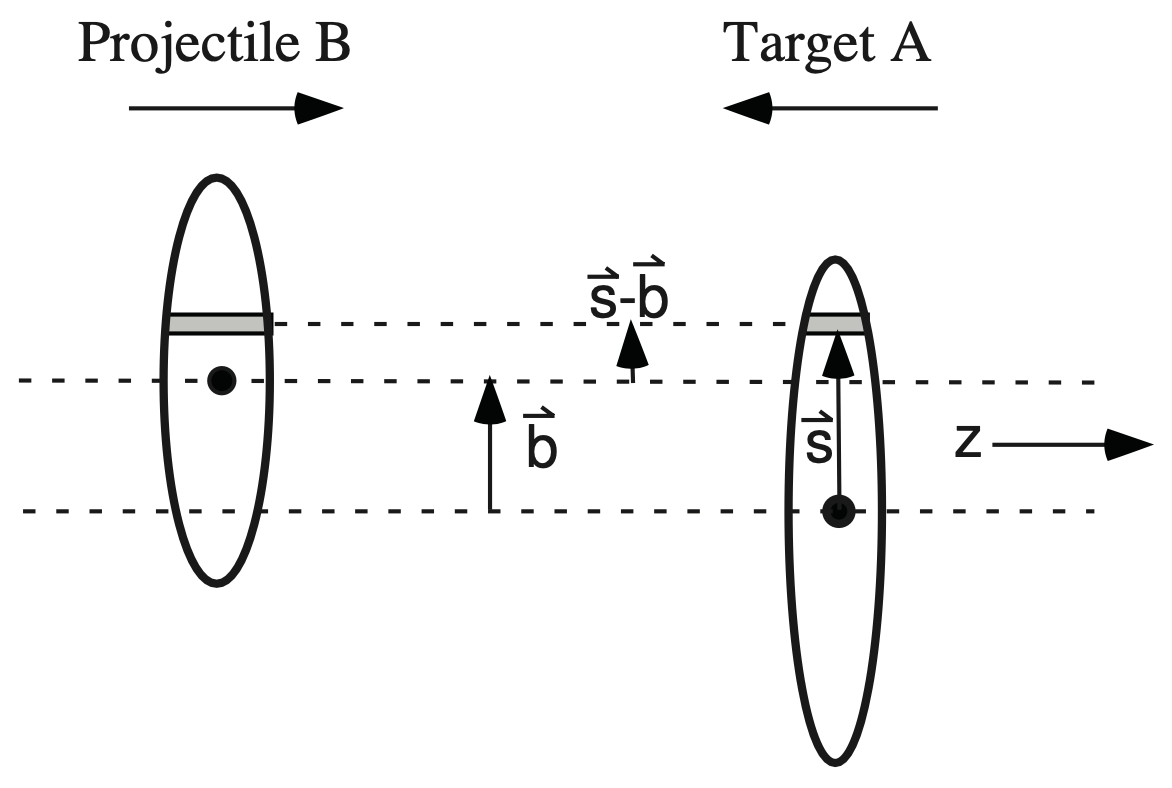
\includegraphics[width=\textwidth]{figures/chapter1/optical_glauber.png}
    \caption{Schematic of the optical limit Glauber model. Reproduced from \cite{glauber_review}.}
    \label{fig:optical_glauber_model}
\end{figure}
The probability of a collision in the overlap region 

\begin{figure}
    \centering
    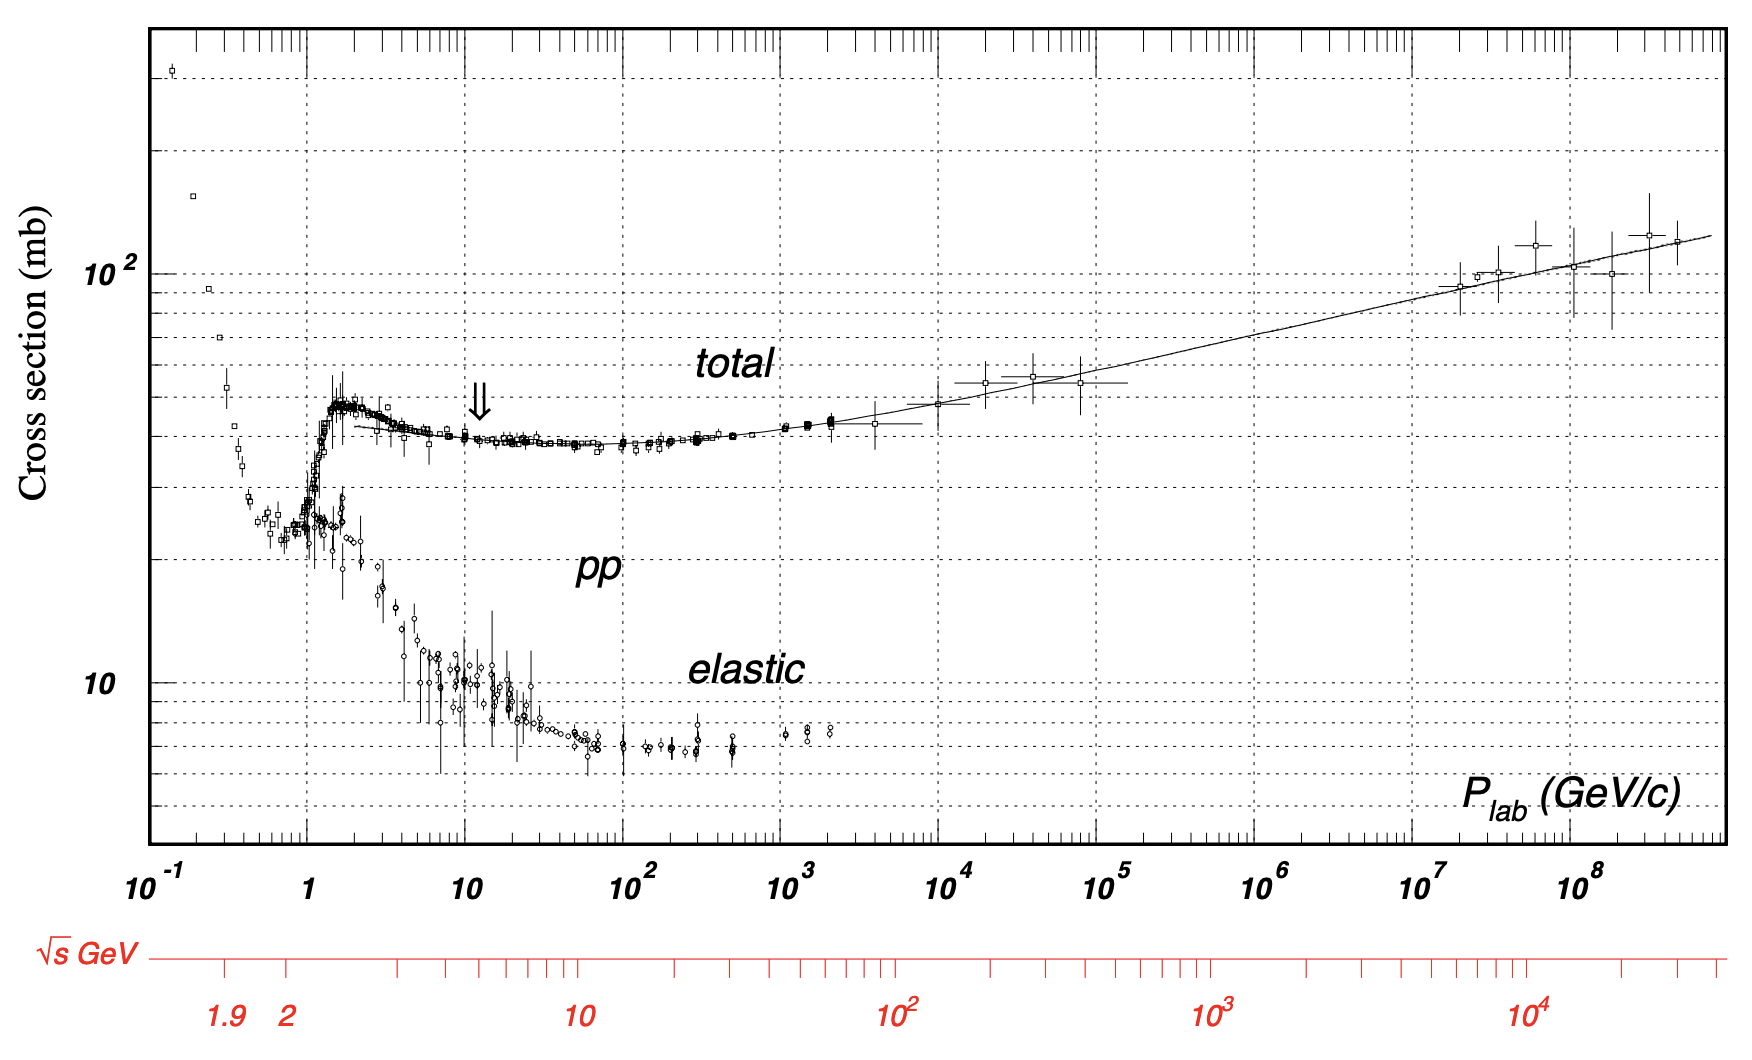
\includegraphics[width=\textwidth]{figures/chapter1/pp_cross_section.png}
    \caption{p+p cross section as a function of collision energy. Reproduced from \cite{ParticleDataGroup:2024cfk}.}
    \label{fig:pp_cross_section}
\end{figure}

The Glauber model was later extended to include a Monte Carlo implementation, which allowed for the modeling of individual nucleon-nucleon collisions rather than continuous matter distributions.
In the Monte Carlo Glauber model, the Woods-Sakon distribution is now sampled to determine the positions of individual nucleons within the colliding nuclei on an event by event basis. 
Figure \ref{fig:mc_glauber_model} shows a schematic of the Monte Carlo Glauber model, where the positions of individual nucleons are sampled from the Woods-Sakon distribution and the collision geometry is determined by the impact parameter, b, which is the transverse distance between the centers of the two colliding nuclei.
Then, the nucleon-nucleon cross section is used to determine if a collision occurs between two nucleons by requiring that the transverse distance between two nucleons be within $\sqrt{\sigma_{NN}/\pi}$, where $\sigma_{NN}$ is the nucleon-nucleon cross section at the given collision energy.
This method allows for the modeling of fluctuations in the initial geometry of the collision and becomes important when comparing to the results from the optical limit model in highly central events.
Additionally, this method includes shadowing effects where interactions with multiple nucleons where nucleons can "hide" behind each other thereby lowering the overall total cross section.
These effects are not included in the optical limit model where the calculation of the total cross section is higher than the measured total cross section.

\begin{figure}
    \centering
    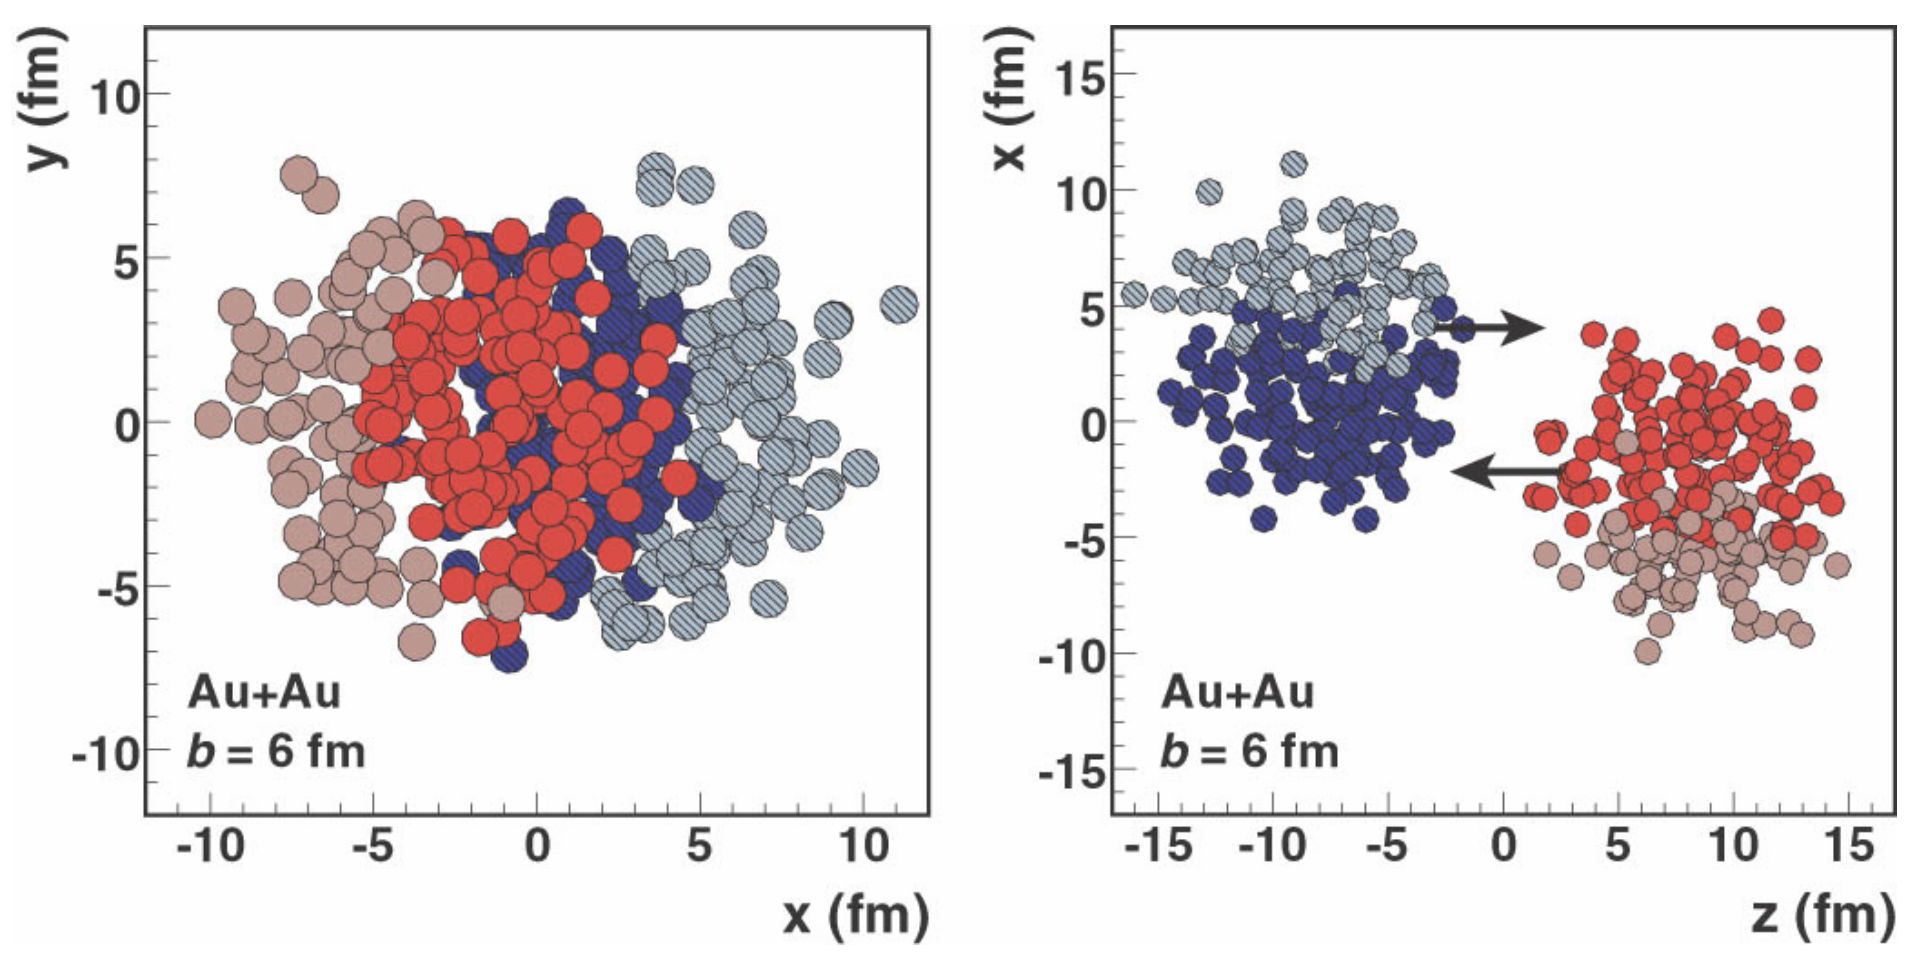
\includegraphics[width=\textwidth]{figures/chapter1/mc_glauber.png}
    \caption{Schematic of the Monte Carlo Glauber model. Reproduced from \cite{glauber_review}.}
    \label{fig:mc_glauber_model}
\end{figure}


\textcolor{red}{Include a figure of the difference between optical limit and MC glauber model.}

\subsubsection{Binary Scaling}

Collisions are tracked between theory and experiment using the number of participant nucleons and number of binary collisions which is something that is calculated from the Glauber model but can also be extracted from experimental measurements using comparisons to the Glauber model.
The number of participant nucleons, $N_{part}$, is the number of nucleons that undergo at least one inelastic collision, and the number of binary collisions, $N_{coll}$, is the total number of inelastic nucleon-nucleon collisions that occur in a given heavy ion collision. 
The number of participant nucleons and number of binary collisions are used to understand the scaling of various observables in heavy ion collisions, such as particle yields and transverse energy, with the geometry of the collision. 
For example, if an observable scales with the number of participant nucleons, it suggests that the observable is primarily influenced by the geometry of the collision and the number of nucleons that are involved in the collision. 
On the other hand, if an observable scales with the number of binary collisions, it suggests that the observable is primarily influenced by hard scatterings between individual nucleons. 

A parameterization of the $N_{part}$ and $N_{coll}$ scaling of various observables including the mean transverse energy as a function of pseudorapidity, \detdeta, has been previously investigated in various collision systems and energies at RHIC. 
The resulting understanding of the scaling of \detdeta with $N_{part}$ and $N_{coll}$ has been found to be well described by a two component model with the form:
\begin{equation}
    \frac{dE_{T}}{d\eta} = A N_{part} + B N_{coll}
\end{equation}
where A and B are free parameters that are fit to the data.
Further studies into the scaling of \detdeta with $N_{pq}$, the number of constituent quark participants, have found that \detdeta scales linearly with $N_{pq}$, suggesting that \detdeta is sensitive to the initial state of the collision \cite{PHENIX_npq_scaling_detdeta}.
\textcolor{red}{Include another statement on \detdeta scaling}.